\section{Evaluation} % (fold)
\label{sec:results}
The energy used by the cluster is a function of the various states that the node is in. The energy usage at various states is usually not a fixed number but a function of time, state and other parameters. S.Dawson-Haggerty et.al.~\cite{Dawson-Haggerty:09} have done a study about the changing power usage of computing nodes with different work loads. The energy usage of a computing node can reasonably be modeled using this equation:
\begin{eqnarray}
    E_{tot}  &= \sum &\big((T_{idle} * E_{idle}) + \nonumber \\
             &       &(T_{waking} * E_{waking}) + \nonumber \\
             &       &(T_{active} * f(E_{active})) + \nonumber \\
             &       &(T_{sleeping} * E_{sleeping}) + \nonumber \\
             &       &(T_{down} * E_{down}) \big)
\end{eqnarray}

\subsection{Experimental Setup} % (fold)
\label{sub:experimental_setup}
All our power measurement experiments were run on a four node Atom cluster. Atom refers to a processor chip from Intel specifically aimed at netbooks. They are hence extremely low powered and energy efficient. We found that the idle power usage of the nodes is about 24W. The nodes take on the order of 2-3 seconds to wake up from sleep (S3) and restore socket bindings. 

\subsubsection{Overhead of CCexec} % (fold)
\label{sub:overhead_of_ccexec}
\begin{figure}[ht]
\centering
\begin{center}
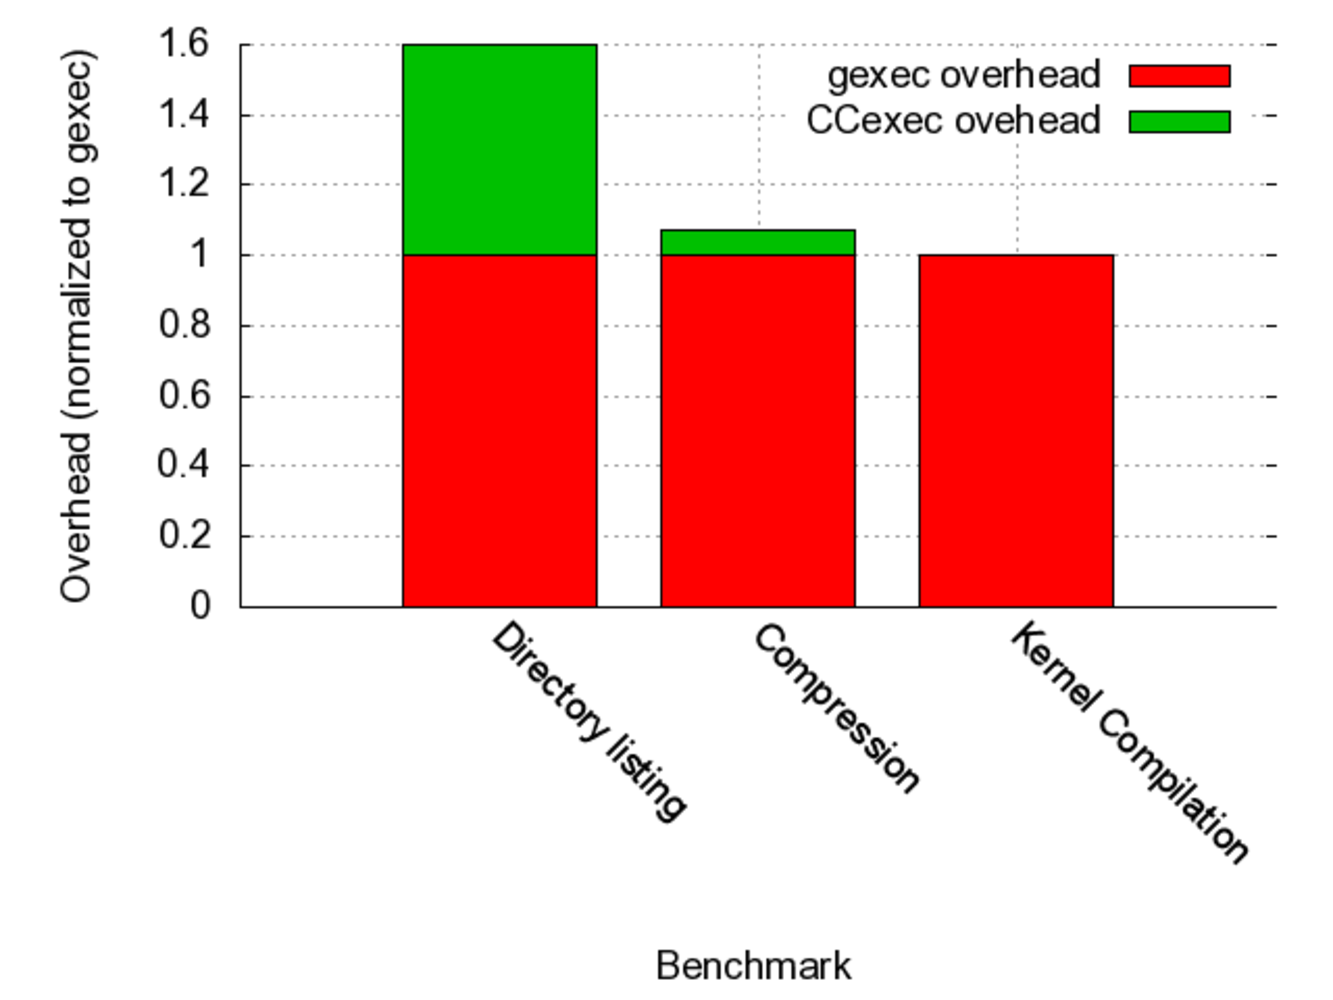
\includegraphics[width=3.0in]{graphs/CCexecVsgexec1.pdf}
\vspace{-0.1in}
\caption{{\normalsize Worst case over head induced by CCexec}\label{fig:ccexec-overhead}}
\vspace{-0.1in}
\end{center}
\end{figure}
\begin{figure}[ht]
\centering
\begin{center}
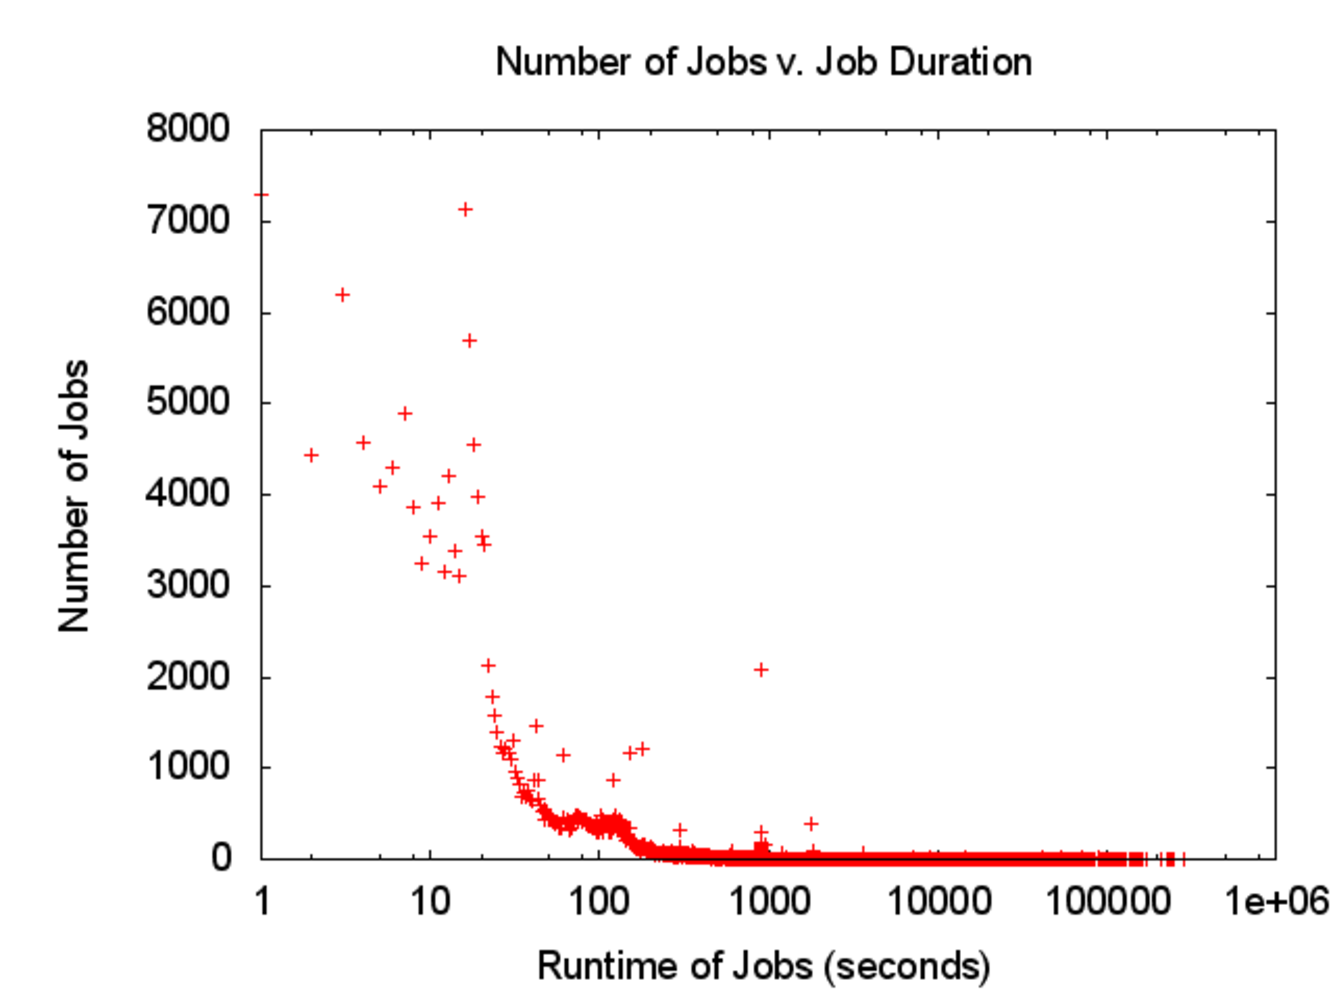
\includegraphics[width=3.0in]{graphs/joblength1.pdf}
\vspace{-0.1in}
\caption{{\normalsize Distribution of Job length in the DAS2 trace}\label{fig:joblength-trace}}
\vspace{-0.1in}
\end{center}
\end{figure}
\begin{figure}[ht]
\centering
\begin{center}
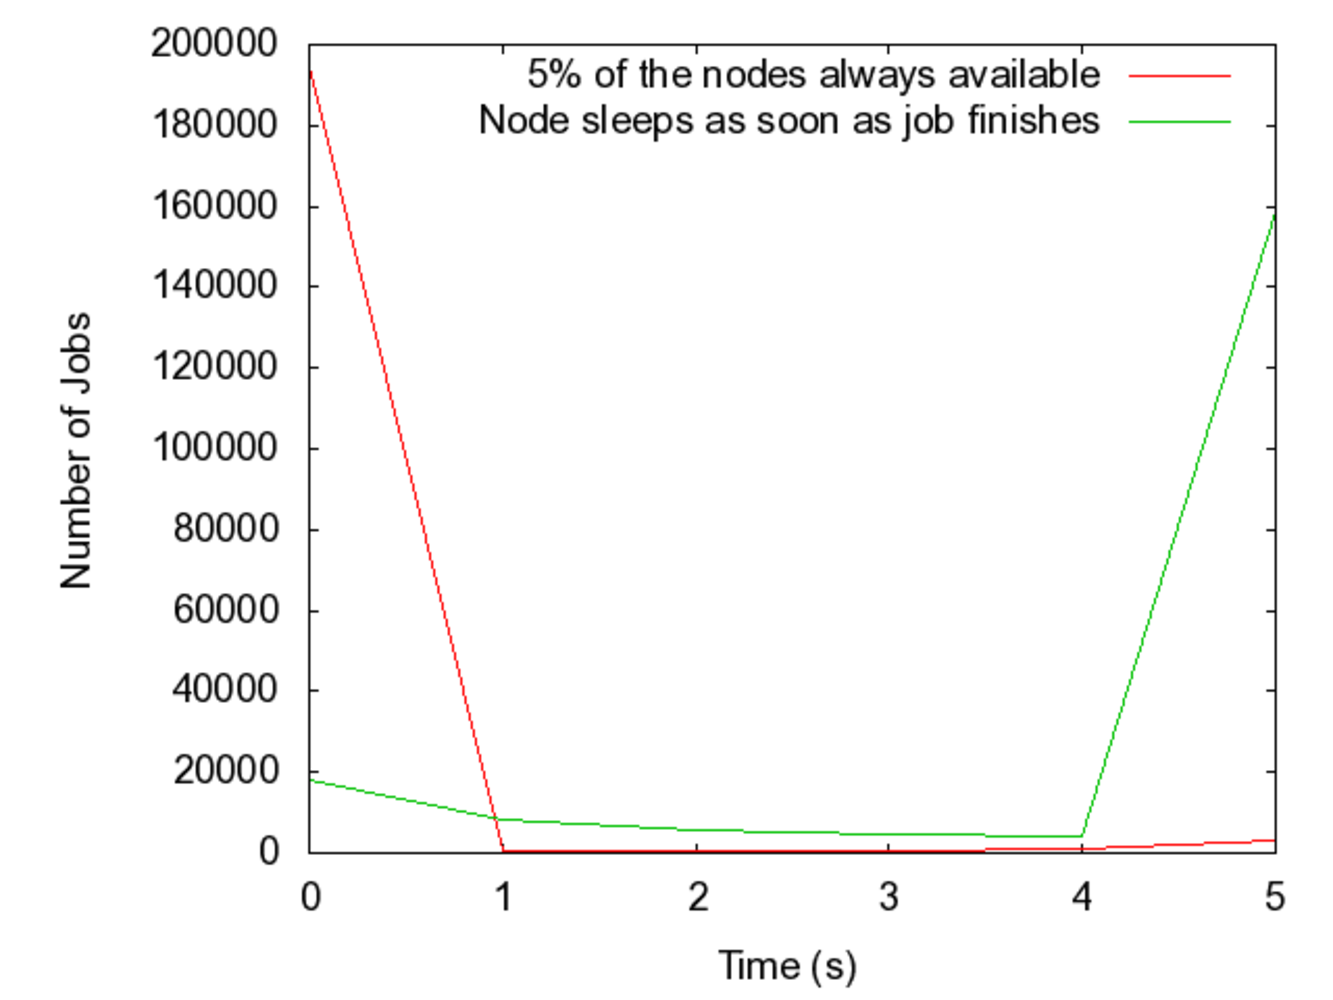
\includegraphics[width=3.0in]{graphs/overhead-time.pdf}
\vspace{-0.1in}
\caption{{\normalsize Distribution of increase in TTC (time to completion) for sleep schedulers}\label{fig:overhead-time}}
\vspace{-0.1in}
\end{center}
\end{figure}
We ran our implementation of CCexec (where all but a single node was sleeping) against gexec (with all nodes awake). This was intended to get an estimate of the worst case performance of CCexec. Intuitively, we expect that all tasks face approximately the same increase in time to completion of the job. Although this is true, it is seen that the performance hit is maximum for quick running jobs, since the overhead is a large percentage of the total runtime of the program. Figure~\ref{fig:ccexec-overhead} details the overhead calculations from our cluster comparing CCexec and gexec. As expected, a short running task like `ls' is about 60\% slower than the gexec counterpart, whereas a typical HPC workload like kernel compilation has an overhead that is barely noticeable. This motivated us to look further into the job distribution in the cluster. Figure~\ref{fig:joblength-trace} shows the job length distribution from the DAS2 cluster. There is a surprisingly large number of short jobs in this trace. It is unsure whether this is an artifact of the cluster being an academic cluster or whether the same behavior is present in industrial clusters. This however requires us to make changes to the naive algorithm of turning nodes on only when needed, as it will adversely affect the short tasks.

% subsection experimental_setup (end)

\subsubsection{Simulator Setup} % (fold)
\label{sub:trace_driven_simulation}
The benchmark results we obtained from our experiments on the Atom node cluster would be a lower bound on the efficiency of compute nodes, since these nodes have minimal power requirements. We use power and timing number reported by the Somniloquy~\cite{Yuvraj:09} for the Dell Optiplex 745 server on traces obtained from the Grid Workload Archive~\cite{gwa}. The values are detailed in Table~\ref{tab:optiplex}.
\begin{description}
    \item[DAS2 5-Cluster Grid Logs] - is a research grid composed of five Pentium/Linux clusters (one cluster with 144 CPUs and the rest with 64). The DAS-2 traces are provided by the Advanced School for Computing and Imaging, the owner of the DAS-2 system.
    \item[Grid 5000 logs] - is an experimental grid platform for large scale parallel and distributed computing research consisting of 9 sites geographically distributed in France. Each site comprises one or  several clusters, for a total of 15 clusters inside Grid 5000.
\end{description}

\begin{table}[tp]
    \label{tab:optiplex}
    \centering
    \begin{tabular}{|c|r|}
        \hline
        {\bf Condition} & {\bf Optiplex 745}\\
        \hline
        Idle Power & 100 W\\
        \hline
        Active Power & 130 W\\
        \hline
        S3 power & 4 W\\
        \hline
        Waking power & 150 W\\
        \hline
        Time to sleep & 9 s\\
        \hline
        Time to wake up & 4 s\\
        \hline
    \end{tabular}
    \caption{Power and timing results for Optiplex 745 server used in evaluation of traces}
\end{table}

Table~\ref{tab:trace-comp} elucidates on the trace details. It also compares the overhead of running the \emph{Naive Sleep} scheduler explained later in Section~\ref{ssub:overhead_induced_by_cc}

\begin{table}
    \centering
    \label{tab:trace-comp}
    \begin{tabular}{|c|r|r|}
        \hline
        & {\bf DAS 2} & {\bf Grid 5000} \\
        \hline
        Trace Length & 192d 15h & 167d 20h\\
        \hline
        No of nodes & 400 & 5000 \\
        \hline
        Active period & 5.68\% & 1.18\% \\
        \hline
        Increase in & 3.66s/41\% & 3.37s/9.8\%\\
        job completion & & \\
        time (Naive Sleep) & &\\
        \hline
    \end{tabular}
    \caption{Comparison of DAS2 and Grid5000 traces}
\end{table}

The simulator is designed to test how different node scheduling algorithms perform on a given job trace. It is written in 1815 lines of Java and is composed of 24 classes. Each class in the simulator represents either information about an actual job, information about a simulated job, or the simulated cluster. The main classes are {\em TraceJob, SimulatedJob, Simulator, Scheduler, NodeProxy, Node} and {\em Command}. 

The simulator begins by creating a list of \emph{TraceJob}s from a trace log (several types of logs are supported). Once this list is created, it is passed into the \emph{Scheduler}. The scheduler uses this list to decide when and how to execute jobs which will be run on the simulator. Jobs become available to be executed once the simulator time passes the actual start time of the job in the trace. The \emph{Simulator} class itself takes as input a \emph{Scheduler} and a list of \emph{Nodes}. For each time step (which is set to 1 second in the tests), the scheduler is polled for a list of \emph{Command}s to execute. A \emph{Command} has the ability to modify the state of the simulator and is the only way the \emph{Scheduler} can modify the state of the nodes. For our purposes, we only use three commands: sleep, wake, and schedule job. % Once the simulator receives the list of commands from the scheduler, the status of the \emph{Nodes} and the \emph{Simulator} are updated for the current time and the Commands received from the Scheduler are executed. 

Since we were mainly concerned with impact of different sleep algorithms on the performance and power consumption of the cluster, it was crucial for the simulator to be easily extensible to test new sleep algorithms and to provide the ability to monitor statistics concerning availability and power usage. For each sleep scheduling algorithm we wanted to test, we created a \emph{NodeProxy} subclass. A \emph{NodeProxy} object is used by the \emph{Scheduler} to get a list of nodes available to run jobs on. This provides a simple way to isolate the sleep scheduling algorithm from the rest of the simulator. % To get useful data about power usage and response, each simulated node was instrumented to store the amount of power is has used and each simulated job stores information about when the job became available and when the job actually started.

% section trace_driven_simulation (end)

\subsection{Sleep scheduling algorithms} % (fold)
\label{ssub:overhead_induced_by_cc}
We evaluate multiple algorithms for scheduling the sleeping of nodes in the cluster and evaluate their effectiveness against the traces. 
\begin{enumerate}
    \item Nodes are woken up only on demand and put to sleep as soon as they finish executing a job (if there are no more jobs waiting to be scheduled). We will call this {\em Naive Sleep}
    \item A certain minimum number of nodes are kept active at all times (evaluation was done for 1\%, 5\% and 10\% of all nodes). We will call this {\em MinNodesActive}.
    \item A certain minimum number of nodes are kept free for new jobs all the time, i.e. when a node is allotted for a job, a new node is woken up to be added to the active queue. (Again evaluation was done for 1\%, 5\% and 10\%). We will call this {\em MinNodesAvail}.
    \item Nodes are kept active for a certain time frame after the current job is finished. This is done with the expectation that job arrival is usually clustered together. We will call this {\em NoImmSleep}.
\end{enumerate}


% subsubsection overhead_induced_by_ccexec (end)
\subsubsection{Simulation Results} % (fold)
\label{ssub:simulation_results}

% subsubsection simulation_results (end)

The DAS2 trace is 192days and 15hours long with over 200000 jobs in the time frame running over 400 CPUs. The baseline energy usage of the cluster for the trace period is 188079 kWh. We compare the effect on energy saving and user experience with various sleep algorithms in Table~\ref{tab:sleep-overhead}. The \emph{MinNodesAvail} with 5\% of nodes available appears to be a good default tradeoff. It saves 81\% of the baseline power while introducing only a 2\% overhead to jobs on average. However, there is a no right scheduler for use in any cluster. It is a performance-power tradeoff that the system administrator would make. As is evident from Figure~\ref{fig:overhead-time}, \emph{MinNodesAvail} at 5\% easily outperforms \emph{Naive Sleep} with respect to user impact.
The trade off between user response and power usage is graphically represented in Figure~\ref{fig:ttc-energy}.

\begin{table*}
    \centering
    \begin{tabular}{|c|c|c|r|r|}
        \hline
        Algorithm & Parameter & Reading & DAS 2 & Grid 5000 \\
        \hline
        \multirow{2}{*}{No Sleep} &  & Energy usage & 188079 kWh & 2021438 kWh \\\cline{3-5}
        & & Avg increase in time to completion & 0\% & 0\% \\
        \hline
        \multirow{2}{*}{Naive Sleep} & & Energy usage & 21084 kWh & 110472 kWh \\\cline{3-5}
        & & Avg increase in TTC & 39.9\% & 9.66\% \\
        \hline
        \multirow{6}{*}{MinNodesActive} & 1\% & Energy usage & 22474 kWh & 128519 kWh\\\cline{3-5}
        & & Avg increase in TTC & 37.4\% & 3.43\% \\\cline{2-5}
        
        & 5\% & Energy usage & 28926 kWh & - \\\cline{3-5}
        & & Avg increase in TTC & 27.8\% & - \\\cline{2-5}
        
        & 10\% & Energy usage & 39827 kWh & - \\\cline{3-5}
        & & Avg increase in TTC & 18.8\% & - \\\cline{2-5}
        \hline
        
        \multirow{6}{*}{MinNodesAvail} & 1\% & Energy usage & 23577 kWh & 142471 kWh \\\cline{3-5}
        & & Avg increase in TTC & 8.6\% & .06\% \\\cline{2-5}
        
        & 5\% & Energy usage & 35865 kWh & 284884 kWh \\\cline{3-5}
        & & Avg increase in TTC & .35\% & 0\% \\\cline{2-5}
        
        & 10\% & Energy usage & 51579 kWh & - \\\cline{3-5}
        & & Avg increase in TTC & .016\% & - \\\cline{2-5}
        \hline
        
        \multirow{6}{*}{NoImmSleep} & 60s & Energy usage & 21661 kWh & 110528 kWh \\\cline{3-5}
        & & Avg increase in TTC & 11.8\% & 6.85\% \\\cline{2-5}
        
        & 300s & Energy usage & 22870 kWh & 110719 kWh \\\cline{3-5}
        & & Avg increase in TTC & 5.95\% & 4.69\% \\\cline{2-5}
        
        & 600s & Energy usage & 23812 kWh & 110930 kWh \\\cline{3-5}142471
        & & Avg increase in TTC & 4.09\% & 3.94\% \\\cline{2-5}
        \hline
    \end{tabular}
    \caption{Measurement of energy and performance overhead of different sleep schedulers on the DAS2 cluster}
    \label{tab:sleep-overhead}
\end{table*}

\begin{figure}[ht]
\centering
\begin{center}
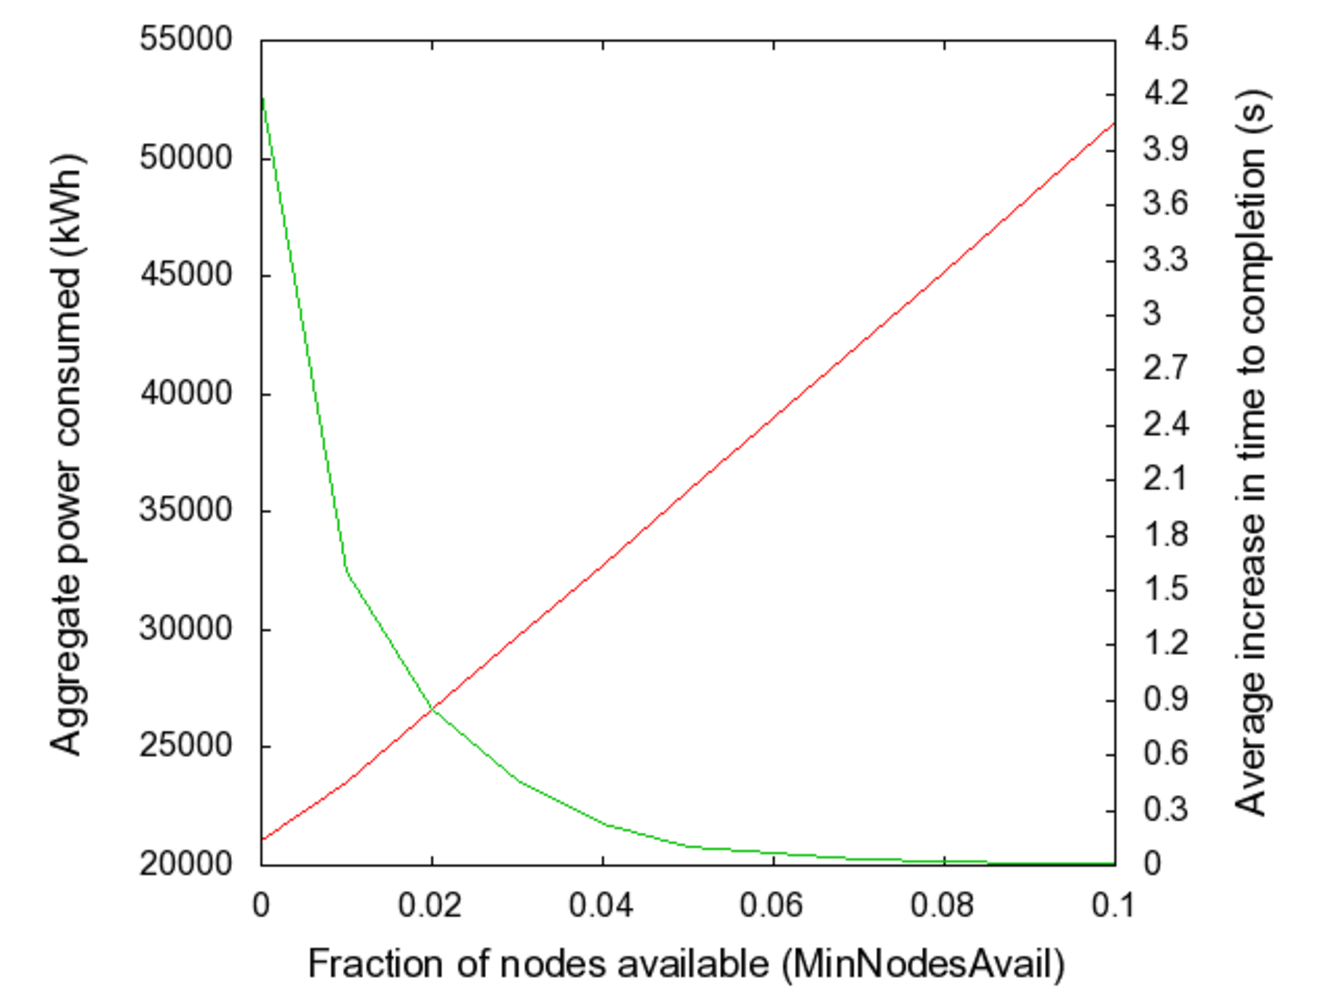
\includegraphics[width=3.0in]{graphs/ttcvsenergy.pdf}
\vspace{-0.1in}
\caption{{\normalsize Energy Vs Response time tradeoff for MinNodesAvail for the DAS2 cluster}\label{fig:ttc-energy}}
\vspace{-0.1in}
\end{center}
\end{figure}

% subsection overhead_of_ccexec (end)

\subsection{Energy saving} % (fold)
\label{sub:energy_saving}
\begin{figure}[ht]
\centering
\begin{minipage}{\linewidth}
\begin{center}
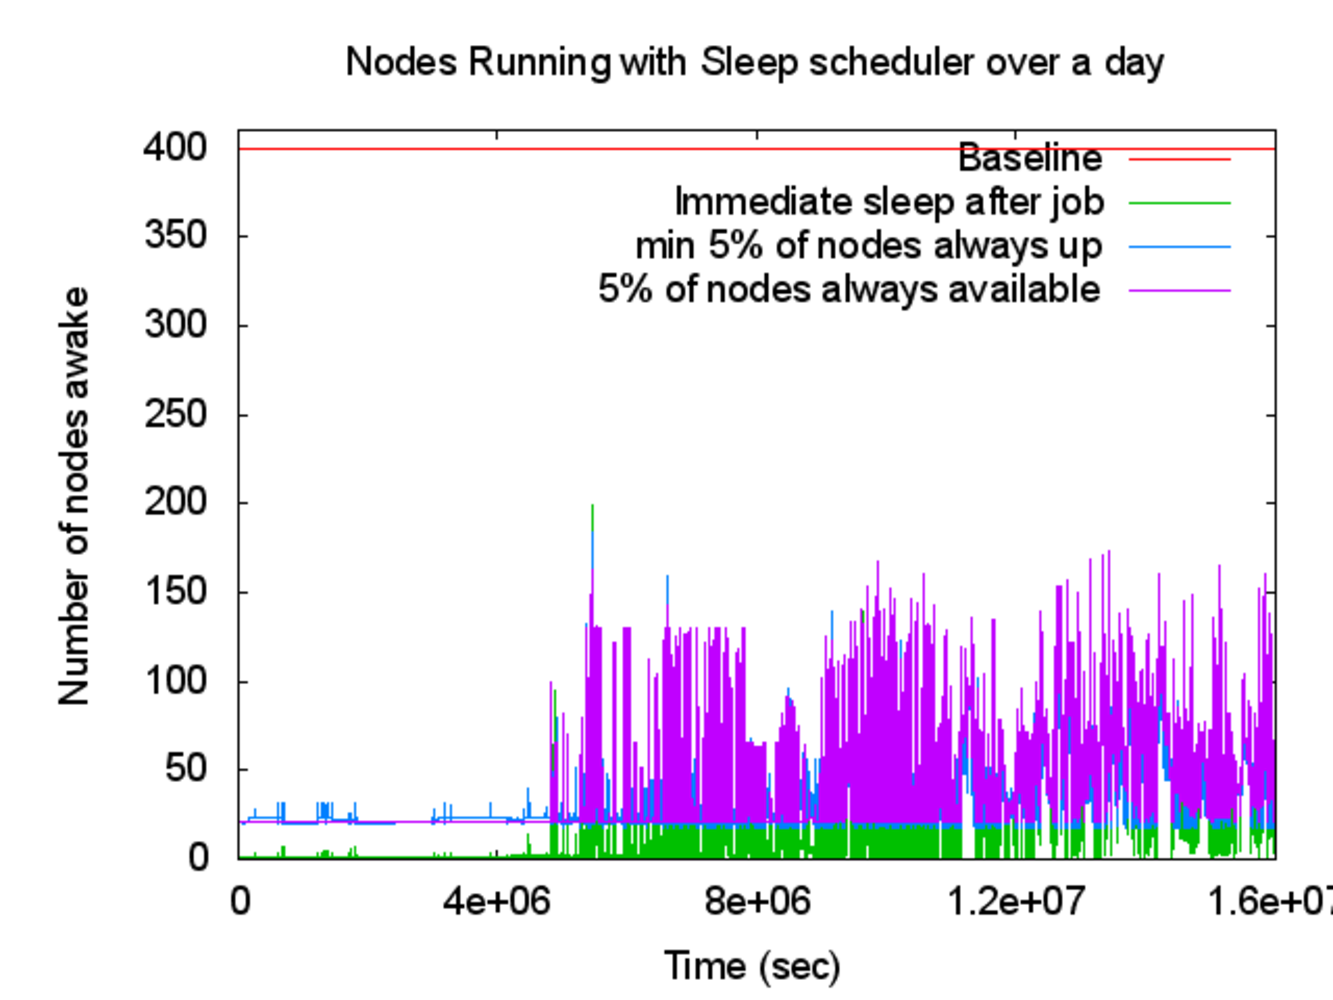
\includegraphics[width=3.0in]{graphs/nodesup1.pdf}
\vspace{-0.1in}
\caption{{\normalsize Set of awake nodes when using CCd over entire  DAS2 cluster trace} \label{fig:nodesup}}
% \vspace{-0.1in}
\end{center}
\end{minipage}
\begin{minipage}{\linewidth}
\begin{center}
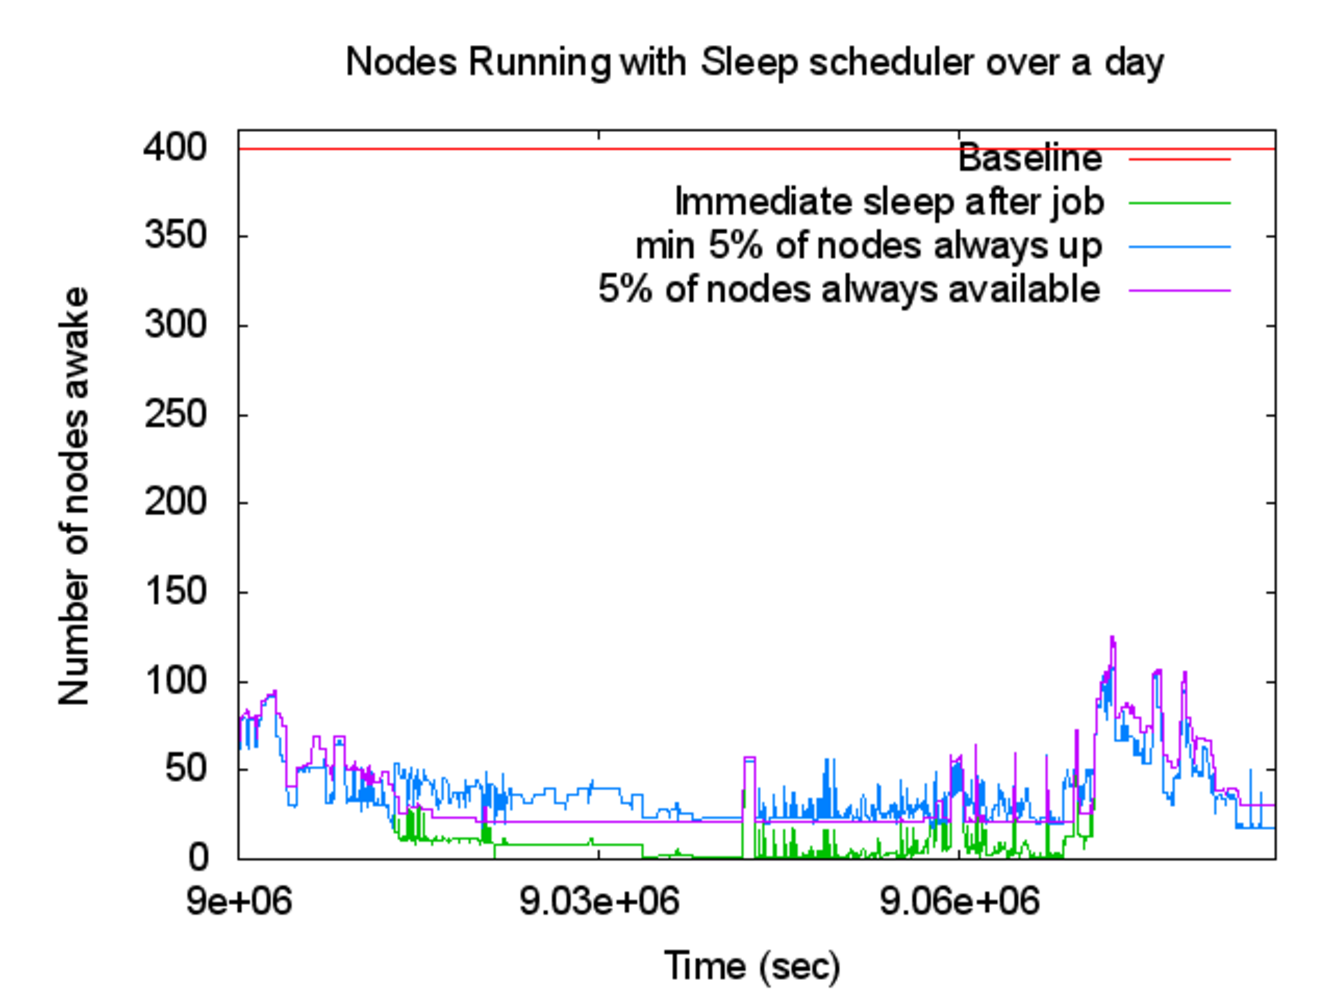
\includegraphics[width=3.0in]{graphs/nodesup-zoomed1.pdf}
\vspace{-0.1in}
\caption{{\normalsize Set of awake nodes on a random day in the DAS2 cluster trace} \label{fig:nodesup-zoomed}}
\vspace{-0.1in}
\end{center}
\end{minipage}
\end{figure}

\begin{figure}[ht]
\centering
\begin{center}
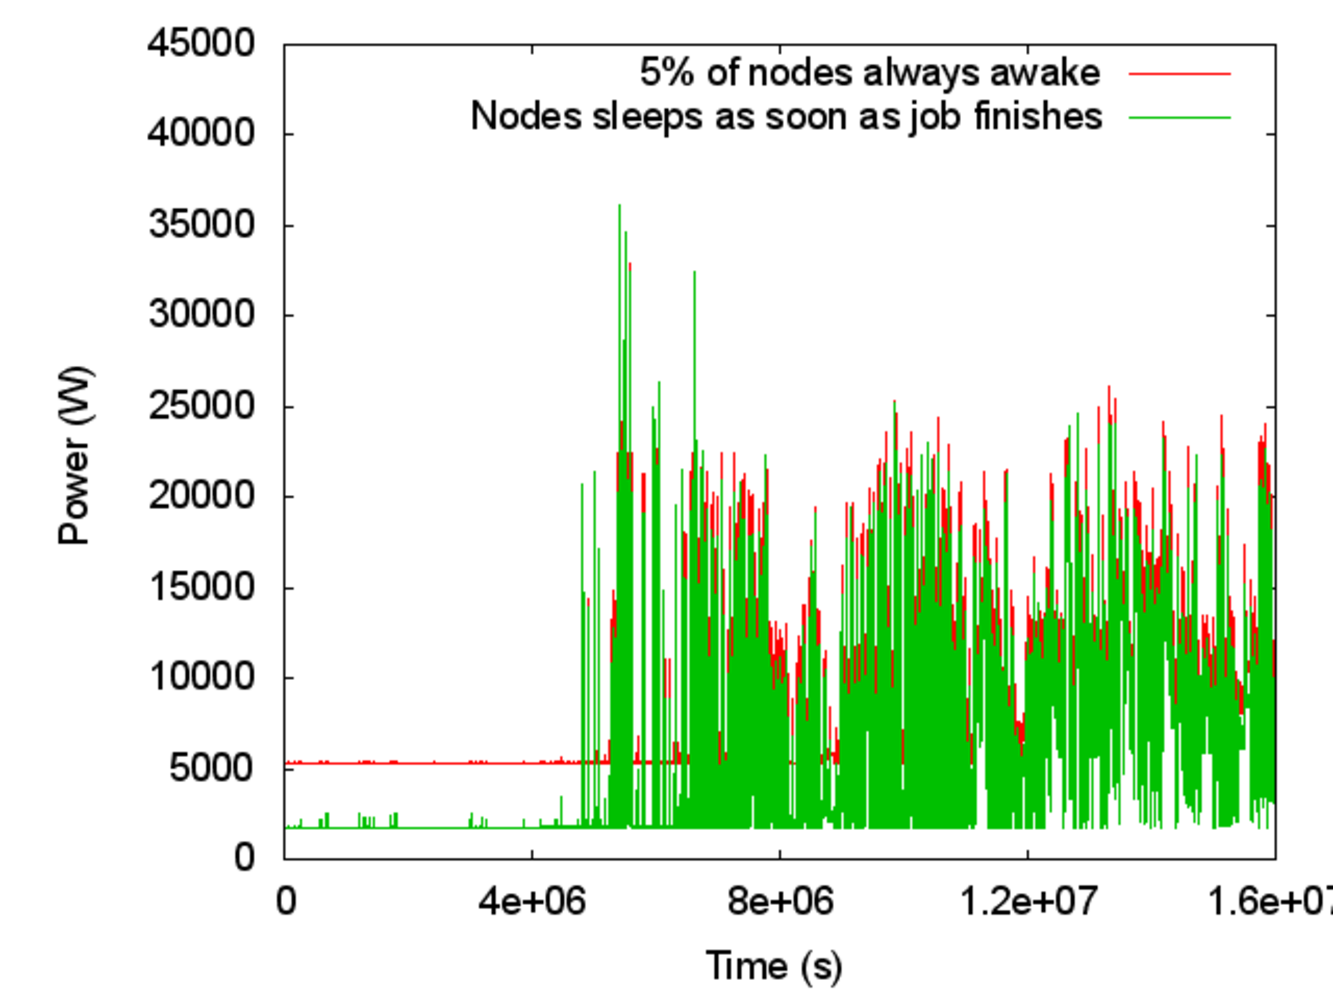
\includegraphics[width=3.0in]{graphs/time-energy.pdf}
\vspace{-0.1in}
\caption{{\normalsize Tradeoff of energy requirements between sleep schedulers}\label{fig:time-energy}}
\vspace{-0.1in}
\end{center}
\end{figure}

\begin{figure}[ht]
\centering
\begin{center}
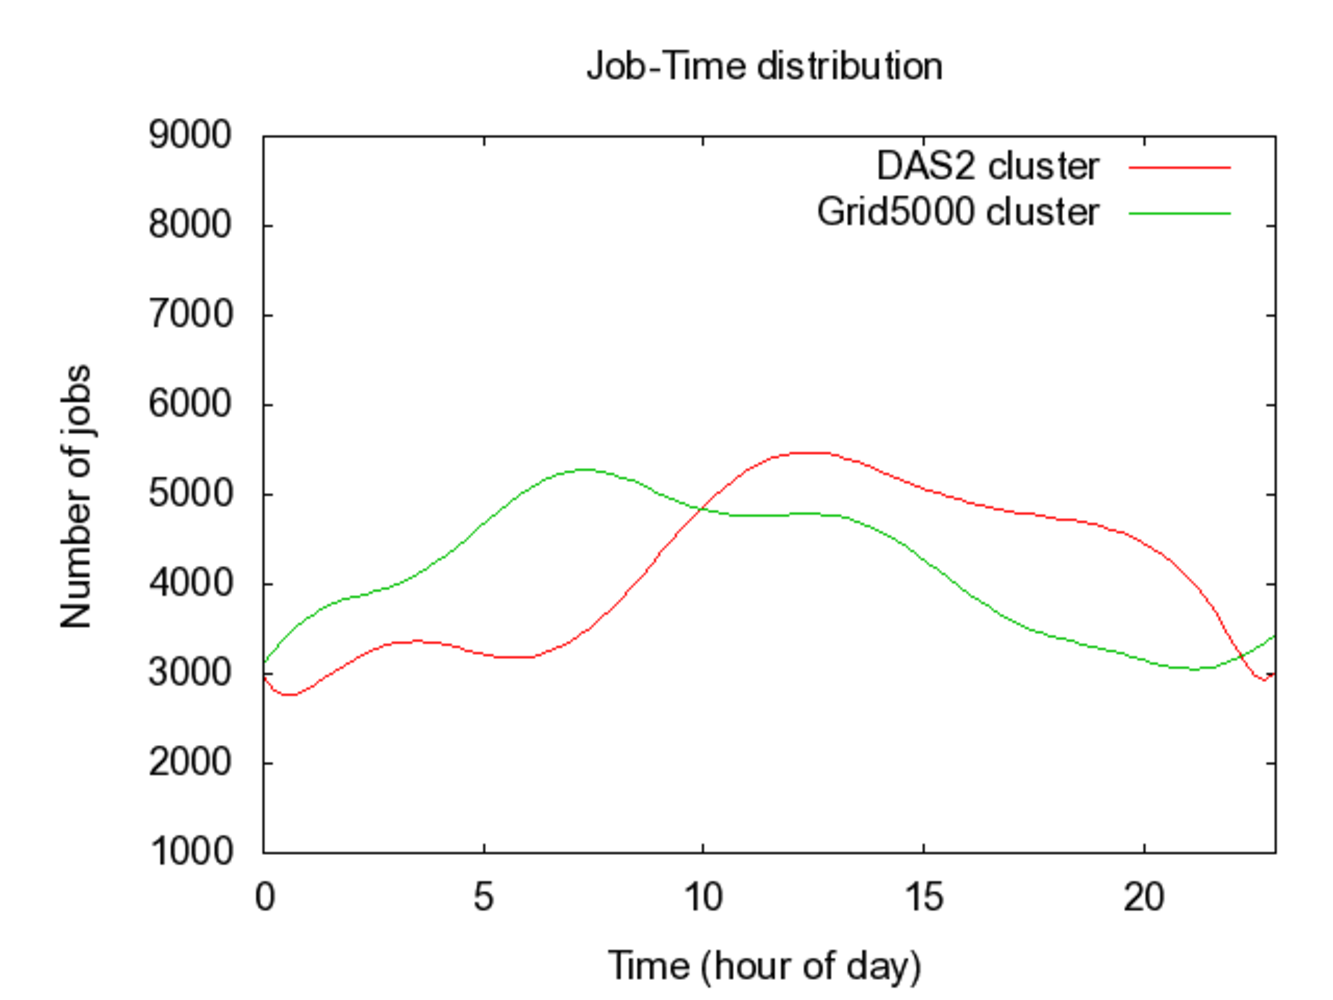
\includegraphics[width=3.0in]{graphs/job-time.pdf}
\vspace{-0.1in}
\caption{{\normalsize Job distribution with hour of day}\label{fig:job-time}}
\vspace{-0.1in}
\end{center}
\end{figure}
% subsection energy_saving (end)
Figure~\ref{fig:nodesup} shows the set of nodes awake at any point of time. The total energy requirements of the cluster is a function of the number of nodes awake at any point in time. Figure~\ref{fig:nodesup-zoomed} is a graph zoomed up to 1 day within Figure~\ref{fig:nodesup}. It is clear that there are periods of time when there is no activity at all and all of the sleep schedulers perform much better than the baseline (no sleeping) of keeping all 400 nodes awake. Figure~\ref{fig:time-energy} compares the cluster energy requirements over the entire DAS2 trace for the \emph{MinNodesAvail} at 5\% scheduler and the \emph{Naive Sleep} scheduler. It can be seen that the \emph{MinNodesAvail} follows quite closely with the \emph{Naive Sleep} scheduler at high utilization times and it is only lacking at time of idleness. Combining this result with the fact that fewer jobs are run in the nights (as seen in Figure~\ref{fig:job-time}), the administrator might choose to have a hybrid approach of \emph{MinNodesAvail} at 1\% at nights and at 5\% in the mornings.


% section results (end)